\documentclass[a4paper,12pt]{article} % добавить leqno в [] для нумерации слева
\usepackage[a4paper,top=1.3cm,bottom=2cm,left=1.5cm,right=1.5cm,marginparwidth=0.75cm]{geometry}
%%% Работа с русским языком
\usepackage{cmap}					% поиск в PDF
\usepackage{mathtext} 				% русские буквы в фомулах
\usepackage[T2A]{fontenc}			% кодировка
\usepackage[utf8]{inputenc}			% кодировка исходного текста
\usepackage[english,russian]{babel}	% локализация и переносы

\usepackage{multirow}
\usepackage{graphicx}
\usepackage{mathtools}
\usepackage{wrapfig}
\usepackage{tabularx}
\usepackage{amssymb}
\usepackage{hyperref}
\usepackage[rgb]{xcolor}
\hypersetup{colorlinks=true,urlcolor=blue}
%% Шрифты
\usepackage{euscript}	 % Шрифт Евклид
\usepackage{amsmath}
\usepackage{mathtools}
%%% Заголовок
\author{Lokhmatov Arseniy}
\title{Лабораторная работа по общей физике}

\date{\today}
\begin{document}
\begin{titlepage}
    \newpage
    \begin{center}
    {\large МОСКОВСКИЙ ФИЗИКО-ТЕХНИЧЕСКИЙ ИНСТИТУТ (НАЦИОНАЛЬНЫЙ ИССЛЕДОВАТЕЛЬСКИЙ УНИВЕРСИТЕТ)}
    \vspace{1cm}

    {\largeФизтех-школа аэрокосмических технологий}
    \vspace{6em}
    \end{center}
    
    \vspace{1.2em}

    \begin{center}
    %\textsc{\textbf{}}
    \Large Лабораторная работа №4.2.1 \\
    Кольца Ньютона
    \linebreak
    \end{center}
    
    \vspace{11em}
    
    \begin{flushright}
                       {\large Работу выполнили\\
                       Лохматов Арсений Игоревич\\
                       Козярский Алексей Сергеевич\\
                       Б03-303 }
    \end{flushright}

    \vspace{\fill}

    \begin{center}
        
\includegraphics[width=0.2\linewidth]{dasr.png}
    \end{center}

    \begin{center}
    Долгопрудный, 2025
    \end{center}

    \end{titlepage}

\section{Теоретическая часть}

\paragraph{В работе используются: } измерительный микроскоп с опак-иллюминатором; плоско выпуклая линза; пластинка из чёрного стекла; ртутная лампа типа ДРШ; щель; линзы; призма прямого зрения; объектная шкала.

Схема экспериментальной установки приведена на рисунке $\ref{img1}$. Опыт выполняется с помощью измерительного микроскопа. На столик микроскопа помещается держатель с полированной пластинкой из чрного стекла. На пластинке лежит исследуемая линза.

\begin{figure}[h]
    \begin{center}
        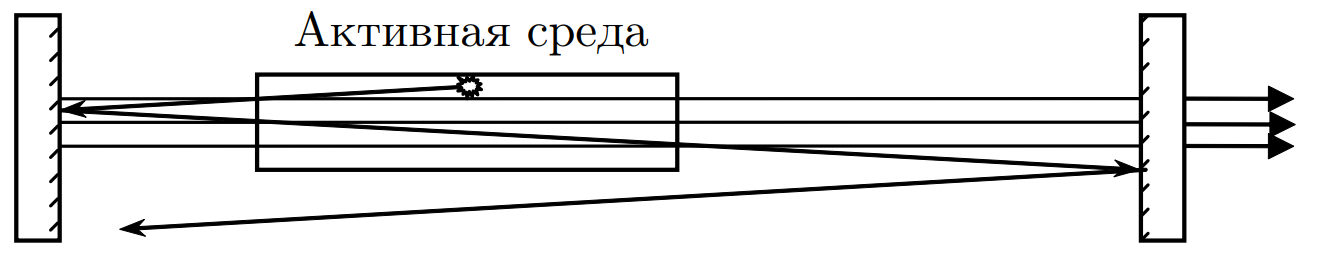
\includegraphics[width=15cm]{image1.png}
    \end{center}
    \caption{Схема экспериментальной установки}
    \label{img1}
\end{figure}

Источником света служит ртутная лампа, находящаяся в защитном кожухе. Для получения монохроматического света применяется призменный монохроматор, состоящий из конденсора $K$, коллиматор (щель $S$ и объектив $O$) и призмы прямого зрения $\text{П}$. Эти устройства с помощью рейтеров располагаются на оптической скамье. Свет от монохроматора попадает на расположенный между объективом и окуляром микроскопа опак-иллюминатор ($\text{ОП}$) -- специальное устройство, служащее для освещения объекта при работе в отражённом свете. Внутри опак-иллюминатора находится полупрозрачная стеклянная пластинка $P$, наклонённая под углом $45^{\circ}$ к оптической оси микроскопа. Свет частично отражается от этой пластинки, проходит через объектив микроскопа и попадает на исследуемый объект. Пластинка может поворачиваться вокруг горизонтальной оси $X$, опак-иллюминатор -- воеруг вертикальной оси.

Столик микроскопа может перемещаться в двух взаимно перпендикулярных направлениях с помощью винтов препаратоводителя. Отсчётный крест окулярной шкалы перемещается перпендикулярно оптичской оси с помощью микрометрического винта $M$.

Оптическая схема монохроматора позволяет получить в плоскости входного окна опак-иллюминатора достаточно хорошо разделённые линии спектра ртутной лампы. Изображение щели $S$ фокусируется на поверхность линзы объективом микроскопа, то есть точка источника и точка наблюдения спектра совпадают. Интерференционная картина не зависит от показателя преломления линзы и определяется величиной зазора между линзой и пластинкой (кольца равной толщины).

\newpage

\section{Практическая часть}

В работе предлагается, измерив диаметры колец Ньютона, определить радиус кривизны линзы; исследовать картину биений и рассчитать разность длин волн между жёлтой и зелёной спектральными линиями ртути.

Установка была отюстирована, микроскоп и монохроматор были настоены, мы сразу приступили к выполнению работы!

\subsection{Измерение диаметров колец}

\begin{enumerate}
    \item Вращая окулярный микрометрический винт, убедились, что перекрестие проходит через центр центрального тёмного пятна, и что поле зрения освещено симметрично слева и справа от центра. При перемещении объектива $O$ ближе к микроскопу вдоль оптической оси, освещённость поля зрения увеличивается.
    \item Установили перекрестие на середину какого-либо достаточно удалённого от центра, но ещё отчётливо видимого тёмного кольца.

    Сняли отсчёт по окулярной шкале: целые деления отсчитывали слева от риски, проходящей через окулрную шкалу, десятые и сотые доли деления - по окулярному микрометрическому винту $M$.

    Для того, чтобы избежать ошибок, возникающих из-за люфта в микрометрическом винте, перекрестие следует подводить к каждому кольцу с одной стороны.

    Перемещая перекрестие, последовательно устанавливали его на середины тёмных и светлых полос и записывали соответствующие показания окулярной шкалы и микрометра. После прохождения через центральное кольцо продолжали измерения, записывая возрастающие номера колец и координаты их диаметров. Резкльтат измерений представлен в таблице $\ref{tab1}$, где $d=|z_1-z_2|$ - диаметр колец.

\begin{table}[h]
    \centering
    \begin{tabular}{|c|c|c|c|}
        \hline
        № & {$z_1$} & {$z_2$} & {$d=|z_1-z_2|$} \\  \hline
         \hline
        1, min  & 7.74 & 0.32 & 7.42 \\ \hline
        1, max  & 7.67 & 0.37 & 7.30 \\ \hline
        2, min  & 7.56 & 0.43 & 7.13 \\ \hline
        2, max  & 7.50 & 0.48 & 7.02 \\ \hline
        3, min  & 7.44 & 0.53 & 6.91 \\ \hline
        3, max  & 7.39 & 0.58 & 6.81 \\ \hline
        4, min  & 7.34 & 0.64 & 6.70 \\ \hline
        4, max  & 7.29 & 0.70 & 6.59 \\ \hline
        5, min  & 7.23 & 0.75 & 6.48 \\ \hline
        5, max  & 7.17 & 0.82 & 6.35 \\ \hline
        6, min  & 7.10 & 0.87 & 6.23 \\ \hline
        6, max  & 7.05 & 0.99 & 6.06 \\ \hline
        7, min  & 6.99 & 1.01 & 5.98 \\ \hline
        7, max  & 6.93 & 1.06 & 5.87 \\ \hline
        8, min  & 6.86 & 1.12 & 5.74 \\ \hline
        8, max  & 6.79 & 1.20 & 5.59 \\ \hline
        9, min  & 6.75 & 1.29 & 5.46 \\ \hline
        9, max  & 6.67 & 1.34 & 5.33 \\ \hline
    \end{tabular}
    \begin{tabular}{|c|c|c|c|}
        \hline
        № & {$z_1$} & {$z_2$} & {$d=|z_1-z_2|$} \\ \hline
        \hline
        10, min & 6.59 & 1.40 & 5.19 \\ \hline
        10, max & 6.52 & 1.45 & 5.07 \\ \hline
        11, min & 6.44 & 1.53 & 4.91 \\ \hline
        11, max & 6.36 & 1.62 & 4.74 \\ \hline
        12, min & 6.28 & 1.71 & 4.57 \\ \hline
        12, max & 6.21 & 1.79 & 4.42 \\ \hline
        13, min & 6.13 & 1.87 & 4.26 \\ \hline
        13, max & 5.98 & 1.95 & 4.03 \\ \hline
        14, min & 5.94 & 2.07 & 3.87 \\ \hline
        14, max & 5.81 & 2.16 & 3.65 \\ \hline
        15, min & 5.73 & 2.27 & 3.46 \\ \hline
        15, max & 5.63 & 2.40 & 3.23 \\ \hline
        16, min & 5.51 & 2.50 & 3.01 \\ \hline
        16, max & 5.37 & 2.68 & 2.69 \\ \hline
        17, min & 5.20 & 2.79 & 2.41 \\ \hline
        17, max & 5.02 & 2.95 & 2.07 \\ \hline
        18, min & 4.86 & 3.11 & 1.75 \\ \hline
        18, max & 4.62 & 3.42 & 1.20 \\ \hline
    \end{tabular}
    \caption{Результаты измерений}
    \label{tab1}
\end{table}

    \item Оценили радиус пятна соприкосновения линзы со стеклянной пластинкой как диаметр центрального минимума: $R\approx1.1$
\end{enumerate}

\subsection{Наблюдение биений}

\begin{enumerate}
    \item Осветили входной окно опак-иллюминатора сразу двумя спектральными компонентами ртути, для этого заменили жёлтый светофильтр на зелёный.

    Получив картину биений, посчитали количество тёмных полос от центра одной чёткой системы полос до центра соседней чёткой системы: $\Delta m=16$.
    
\end{enumerate}

\subsection{Калибровка окулярной шкалы}

\begin{enumerate}
    \item Для определения цены деления окулярной шкалы положили сверху на линзу калиброванную объектную шкалу. Плавно поднимая тубус микроскопа, настроились на стеклянную поверхность шкалы. Перемещая столик, нашли изображение миллиметровой шкалы, совместили его с окулярной шкалой и добились наибольшей чёткости.

    Объектная шкала размером $1 \text{ мм}$ разбита на $100$ делений.

    Используявсё поле зрения микроскопа, отметили самые удалённые друг от друга штрихов объектной шкалы, которые лучше всего совпадают со штрихами окулярной шкалы. В итоге, на $8$ делений окулярной шкалы приходится $0,79\text{ мм}$ объектной шкалы.
\end{enumerate}

\subsection{Обработка результатов}

\begin{enumerate}
    \item Рассчитали цену деления окулярной шкалы о ценили погрешность результата как ошибка объектной шкалы:

    \[ \Delta=\frac{790}{8}\text{ мкм}\approx(98.8\pm0.9)\text{ мкм}. \]

    \item Рассчитали разность длин волн для жёлтой ($\lambda_{\text{жёлтый}}=5780\text{ A}$) и зелёной ($\lambda_{\text{зелёный}}=5461\text{ A}$) линий ртути, полученную при наблюдении биений:

    \[ \Delta\lambda=\frac{\lambda_{\text{зелёный}}}{\Delta m}=\frac{5461}{16}=341\text{ A}. \]

    В теории же должно получиться $\Delta\lambda^{\text{theory}}=5780\text{ A}-5461\text{ A}=319\text{ A}$.
    
    \item Рассчитали радиусы тёмных и светлых полос и построили графики зависимостей $r^2_{m}$ и $(r'_{m})^2$ от номера кольца $m$. На графике так же указана граница тёмного центрального пятна. Через начало координа должен проходить график $r_{m}^2(m)$, потому что центральное пятно -- тёмное. Полученный график представлен на рисунке $\ref{img2}$.

    \begin{figure}[h]
        \begin{center}
            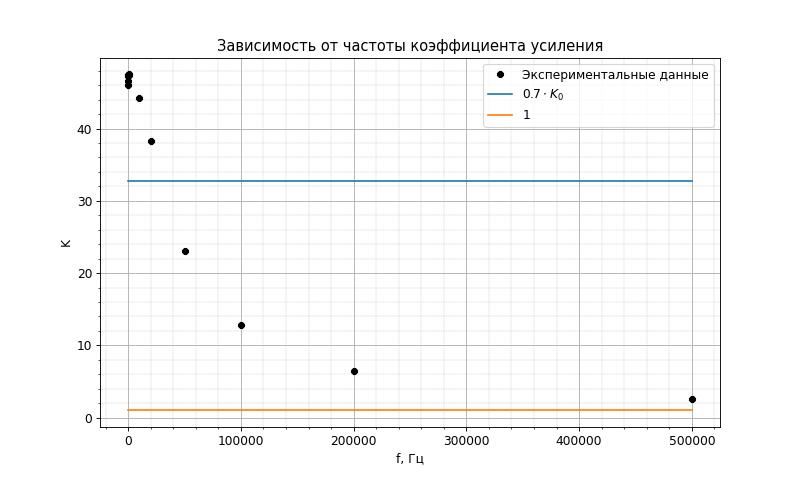
\includegraphics[width=18cm]{image2.jpg}
        \end{center}
        \caption{График зависимости $r^2_{m}$ и $(r'_{m})^2$ от номера кольца $m$}
        \label{img2}
    \end{figure}

    \item Зная длину волны $\lambda=5461 A$, по наклону прямой, проходящей через точки минимума, рассчитаем радиус $R$ кривизны линзы.

    \[ k_{min} = (3.672\pm0.016)\cdot10^{-3}\text{ мм}^2, \]
    \[ r_m=\sqrt{m\lambda R} \Leftrightarrow r_{m}^2 = km, \text{ где } k = k_{min}=\lambda R, \]
    \[  \Longrightarrow R=\frac{k_{min}}{\lambda} = \frac{3.672\cdot10^{-3}}{5461\cdot10^{-7}}=6.72\text{ мм} \]

    \item Оценим погрешность результата, которая напрямую зависит от погрешности определения угла наклона полученного графика:

    \[ \delta R=R\cdot\sqrt{\bigg(\frac{\delta k}{k}\bigg)^2} = R\frac{\delta k}{k} = 6.7\cdot\frac{0.016}{3.672} = 0.03\text{ мм} \]
    
\end{enumerate}

\section{Подведение итогов и выводы}

В ходе данной работы мы исследовали кольца Ньютона, измерили диавметры этих колец и определили радиус кривизны линзы:

\[ R = (6.72\pm0.03)\text{ мм}. \]

Так же мы исследовали рартину биений и рассчитали разность длин волн между зелёной и жёлтой спектральными диниями ртути. Полученный результат совпадает по порядку величины с табличным, но отличается от него (отклонение составляет $\varepsilon=6.9\%$), что говорит о том, что при измерении наш глаз не смог различить ещё несколько тёмных полос.

\end{document}
